\documentclass{beamer}

\mode<presentation> {

% The Beamer class comes with a number of default slide themes
% which change the colors and layouts of slides. Below this is a list
% of all the themes, uncomment each in turn to see what they look like.

%\usetheme{default}
%\usetheme{AnnArbor}
%\usetheme{Antibes}
%\usetheme{Bergen}
%\usetheme{Berkeley}
%\usetheme{Berlin}
%\usetheme{Boadilla}
%\usetheme{CambridgeUS}
%\usetheme{Copenhagen}
%\usetheme{Darmstadt}
%\usetheme{Dresden}
%\usetheme{Frankfurt}
%\usetheme{Goettingen}
%\usetheme{Hannover}
%\usetheme{Ilmenau}
%\usetheme{JuanLesPins}
%\usetheme{Luebeck}
\usetheme{Madrid}
%\usetheme{Malmoe}
%\usetheme{Marburg}
%\usetheme{Montpellier}
%\usetheme{PaloAlto}
%\usetheme{Pittsburgh}
%\usetheme{Rochester}
%\usetheme{Singapore}
%\usetheme{Szeged}
%\usetheme{Warsaw}

% As well as themes, the Beamer class has a number of color themes
% for any slide theme. Uncomment each of these in turn to see how it
% changes the colors of your current slide theme.

%\usecolortheme{albatross}
%\usecolortheme{beaver}
%\usecolortheme{beetle}
%\usecolortheme{crane}
%\usecolortheme{dolphin}
%\usecolortheme{dove}
%\usecolortheme{fly}
%\usecolortheme{lily}
%\usecolortheme{orchid}
%\usecolortheme{rose}
%\usecolortheme{seagull}
%\usecolortheme{seahorse}
%\usecolortheme{whale}
%\usecolortheme{wolverine}

%\setbeamertemplate{footline} % To remove the footer line in all slides uncomment this line
%\setbeamertemplate{footline}[page number] % To replace the footer line in all slides with a simple slide count uncomment this line

%\setbeamertemplate{navigation symbols}{} % To remove the navigation symbols from the bottom of all slides uncomment this line
}

\usepackage{graphicx} % Allows including images
\usepackage{booktabs} % Allows the use of \toprule, \midrule and \bottomrule in tables
\usepackage[spanish]{babel}
\usepackage{thumbpdf}
\usepackage{wasysym}
\usepackage{ucs}
\usepackage[utf8]{inputenc}
\usepackage{pgf,pgfarrows,pgfnodes,pgfautomata,pgfheaps,pgfshade}
\usepackage{verbatim}
\usepackage{multicol}	
\usepackage{url}
\usepackage{mathtools}
\usepackage{tabularx}
\usepackage{listings}
%----------------------------------------------------------------------------------------
%	TITLE PAGE
%----------------------------------------------------------------------------------------

\title[GEYKE93]{Crytography library} % The short title appears at the bottom of every slide, the full title is only on the title page

\author{Gabriel Jiménez B23466 \\ Carla Vega B06763} % Your name
\institute[UCR] % Your institution as it will appear on the bottom of every slide, may be shorthand to save space
{
University of Costa Rica \\ % Your institution for the title page
\medskip
\textit{}
}
\date{October 7th, 2013} % Date, can be changed to a custom date \today

\begin{document}

\begin{frame}
\titlepage {} % Print the title page as the first slide
\end{frame}

\begin{frame}
\frametitle{Overview} % Table of contents slide, comment this block out to remove it
\tableofcontents % Throughout your presentation, if you choose to use \section{} and \subsection{} commands, these will automatically be printed on this slide as an overview of your presentation
\end{frame}

%----------------------------------------------------------------------------------------
%	PRESENTATION SLIDES
%----------------------------------------------------------------------------------------

%------------------------------------------------
\section{Introduction}
\begin{frame}
\frametitle{History}
\begin{itemize}
\item Julio César
\item XV León Battista Alberti 
\begin{itemize}
\item 1470 Tratado de Cifras
\item 1530 Poligraphy
\end{itemize}
\item XVI Girolamo Cardano
\item XIX Transposition
\item 1919 Alexander Koch and Arthur Sherbius (ENIGMA) 1st patent
\item 1975 Diffie and Hellman public key algorithms
\end{itemize}
\end{frame}

\begin{frame}
\frametitle{Cryptology}
Combined study of cryptography and cryptanalysis
\begin{itemize}
\item Cryptoanalysis: study of how to crack encryption algorithms or their implementations.
\item Cryptography: use and practice of cryptographic techniques.
\begin{itemize}
\item "hidden, secret"; and graphein, "writing".
\end{itemize}
\end{itemize}
\begin{figure}
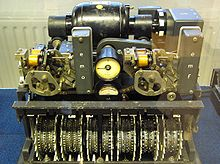
\includegraphics[width=0.3\linewidth]{ww2.jpg}
\caption{German Lorenz cipher machine}
\label{F:German Lorenz cipher machine}
\end{figure}
\end{frame}

\begin{frame}
\frametitle{Classic criptography}
\begin{itemize}
\item Sustitution: Cesar algorithm (A becomes D, B becomes C...), ROT13, ROT47, Vigénere 
\item Transposition: random order
\begin{figure}
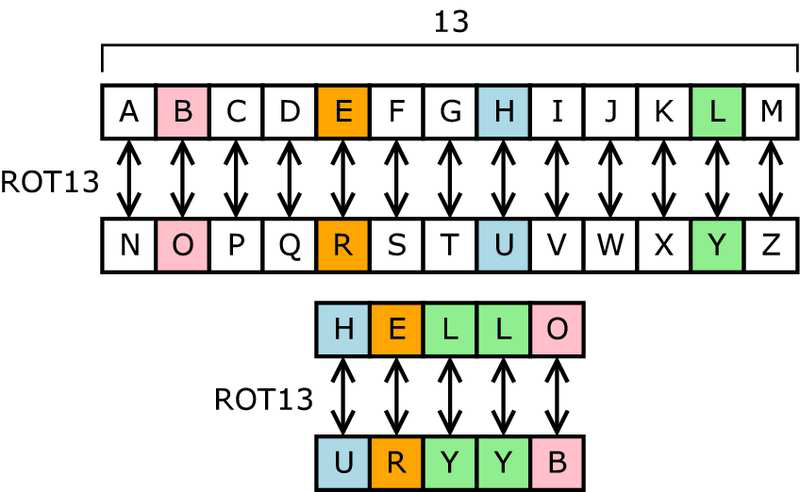
\includegraphics[width=0.6\linewidth]{rot13.png}
\end{figure}
\end{itemize}
\end{frame}

\begin{frame}
\frametitle{Criptography algorithm}
\begin{itemize}
\item Simetric or convencional cryptosystem
\item Asimetric or public key cryptosystem
\end{itemize}
\end{frame}

\begin{frame}
\frametitle{Criptography algorithm}
\framesubtitle{Simetric cryptosystem}
\begin{itemize}
\item Polyalphabetic Cipher: Enigma, Purple, SIGABA, TypeX
\item Stream Cipher (Cifrado de lujo): RC4, Chameleon, FISH, Helix, ISAAC, Panama, Pike, SEAL, SOBER, WAKE
\item Block Cipher: DES, AES, IDEA, Skipjack, Blowfish, RC2, RC5, CAST-128
\end{itemize}
\end{frame}

\begin{frame}
\frametitle{Criptography algorithm}
\framesubtitle{Simetric cryptosystem}
\begin{figure}
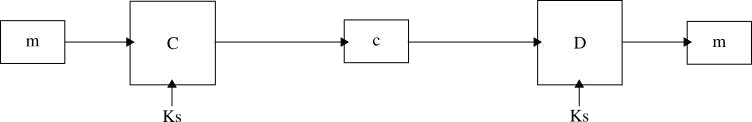
\includegraphics[width=0.8\linewidth]{cp.png}
\end{figure}
\end{frame}

\begin{frame}
\frametitle{Criptography algorithm}
\framesubtitle{Asimetric cryptosystem}
\begin{itemize}
\item Diffie-Hellman
\item RSA
\item DSA (Digital signature algorithm)
\item ElGamal
\item ECC (Criptografía de curva elíptica)
\end{itemize}
\begin{figure}
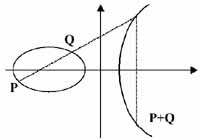
\includegraphics[width=0.4\linewidth]{ecc.png}
\end{figure}
\end{frame}

\section{GEYKE93}
\begin{frame}
\frametitle{GEYKE93 contents}
\begin{itemize}
\item AES
\item RSA
\item Hash function: MD5, SHA256, SHA512
\end{itemize}
\end{frame}


\subsection{AES}

\begin{frame}
\frametitle{AES}
\framesubtitle{Advanced Encryption Standard}
\begin{itemize}
\item Rijndael (Joan Daemen y Vincent Rijmen, Katholieke Universiteit Leuven)
\item 1998
\item Key sizes: 128, 192 or 256 bits
\item Structure: Substitution-permutation network
\end{itemize}
\end{frame}

\begin{frame}
\frametitle{AES}
\begin{figure}
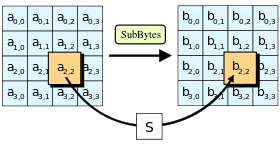
\includegraphics[width=0.6\linewidth]{aes.png}
\end{figure}
\end{frame}

\subsection{RSA} % A subsection can be created just before a set of slides with a common theme to further break down your presentation into chunks

\begin{frame}
\frametitle{RSA}
\begin{columns}[c] % The "c" option specifies centered vertical alignment while the "t" option is used for top vertical alignment

\column{.45\textwidth} % Left column and width
\begin{figure}
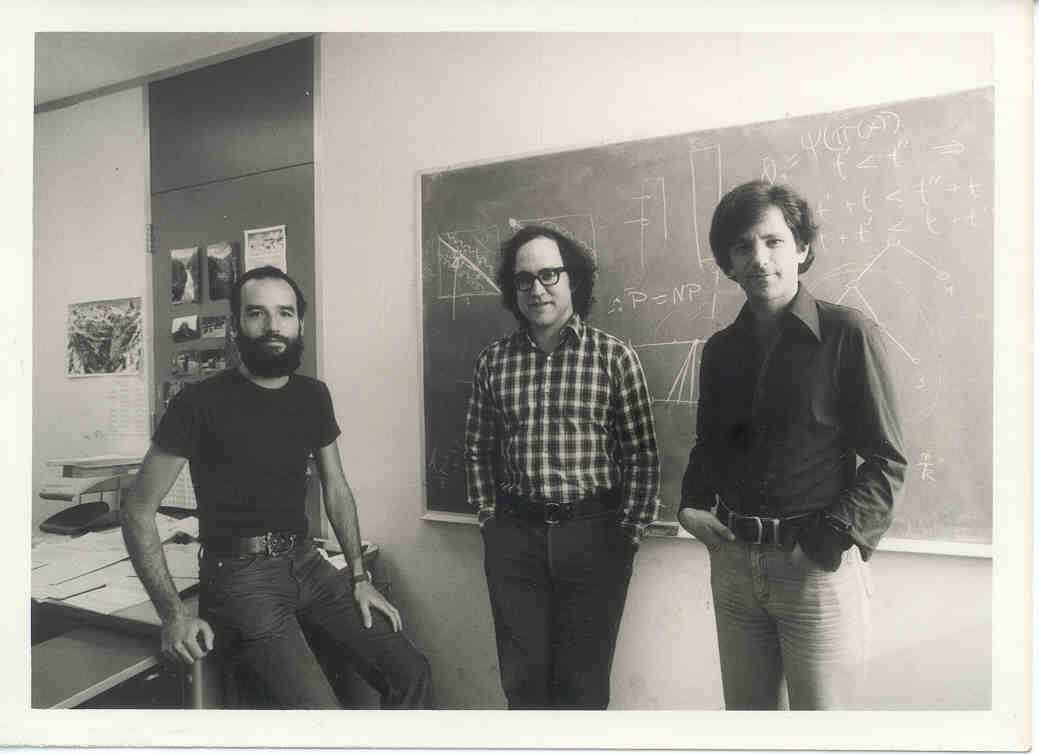
\includegraphics[width=0.9\linewidth]{rsa.png}
\end{figure}

\column{.5\textwidth} % Right column and width
\begin{itemize}
\item Ron Rivest, Adi Shamir, Len Adleman (MIT, 1977)
\end{itemize}
\begin{figure}
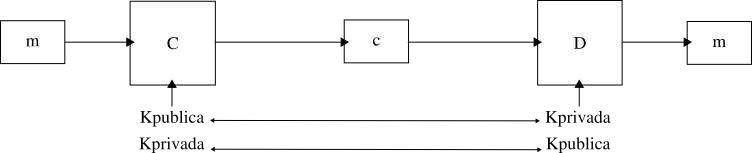
\includegraphics[width=0.9\linewidth]{cpri.png}
\end{figure}
\end{columns}
\end{frame}

\begin{frame}[fragile]
\frametitle{RSA}
\begin{itemize}
\item $(M,C,K,E,D)$
\item $(C_{i} ,D_{i})$
\item $N= PQ$
\item $f = \varphi (N ) = (P − 1)(Q − 1)$
\item $E$ Euclides Algorithm (m.c.d)
\item Public key (E, N)
\item $DE \equiv  1(mod f )$
\item Private key = D
\item $C \equiv  M^{E }(mod N )$
\item $M \equiv  { C}^{D } (mod N )$
\end{itemize}
\end{frame}

\subsection{Hash function}
\begin{frame}
\frametitle{Hash function}
\begin{itemize}
\item Digital sign
\item Fingerprint or digest
\item Algorithm: HAVAL, MD2 (Message digest algorithm), MD4, MD5, SHA0, SHA1, SHA2, SHA3*, Snefru, Tiguer, Whirlpool 
\end{itemize}
\begin{figure}
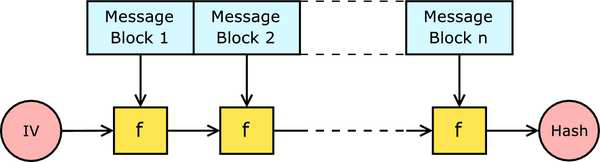
\includegraphics[width=0.6\linewidth]{hash.png}
\end{figure}
\end{frame}

\begin{frame}
\frametitle{Hash function}
\begin{figure}
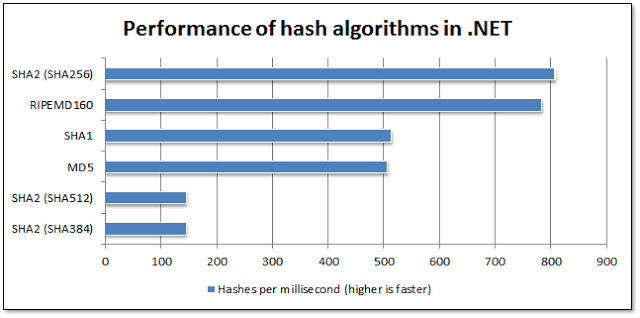
\includegraphics[width=0.9\linewidth]{comp.png}
\end{figure}
\end{frame}

\subsubsection{MD5}

\begin{frame}
\frametitle{MD5}
\framesubtitle{Message digest algorithm}
\begin{itemize}
\item Produces a 128-bit (16-byte) hash value
\item Ron Rivest (1991): replace an earlier hash function, MD4.
\item MD5 hash value is typically expressed as a hexadecimal number, 32 digits long.
\end{itemize}
\end{frame}

\begin{frame}
\frametitle{Attack}
\begin{enumerate}
\item A 2009 attack by Tao Xie and Dengguo Feng breaks MD5 collision resistance in $2^{20,96}$ time. This attack runs in a few seconds on a regular computer.
\item GPUs:
\begin{itemize}
\item NVIDIA GeForce 8400GS graphics processor, 16–18 million hashes per second can be computed. 
\item NVIDIA GeForce 8800 Ultra can calculate more than 200 million hashes per second.
\end{itemize}
\end{enumerate}
\end{frame}

\begin{frame}
\frametitle{MD5}
\begin{columns}[c] % The "c" option specifies centered vertical alignment while the "t" option is used for top vertical alignment

\column{.45\textwidth} % Left column and width
\begin{figure}
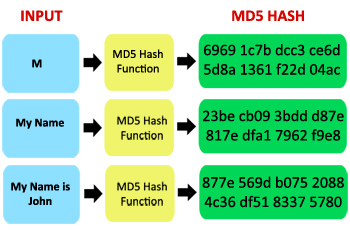
\includegraphics[width=0.8\linewidth]{md5.jpg}
\end{figure}

\column{.5\textwidth} % Right column and width
\begin{figure}
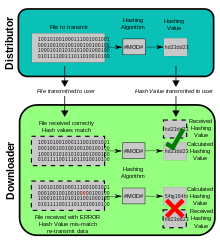
\includegraphics[width=0.8\linewidth]{diagram-md5.png}
\end{figure}
\end{columns}
\end{frame}

\subsubsection{SHA2}

\begin{frame}
\frametitle{SHA2}
\begin{itemize}
\item SHA256: 32-bit words
\item SHA512: 64-bit words
\end{itemize}
\end{frame}

\begin{frame}
\frametitle{SHA2}
\begin{itemize}
\item SHA0 160-bit hash function (1993).
\item SHA1 National Security Agency (NSA) 2010.
\item SHA2 National Institute of Standards and Technology (NIST) as a U.S. Federal Information Processing Standard (FIPS) 2001.
\item Truncated versions of each standardized, known as SHA-224 and SHA-384 (NSA).
\item SHA3 (Keccak, 2012) public competition among non-NSA designers. Same hash lengths as SHA2, and its internal structure differs significantly.
\end{itemize}
\end{frame}

\begin{frame}
\frametitle{SHA2}
\begin{figure}
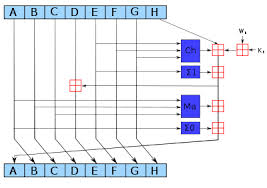
\includegraphics[width=0.8\linewidth]{sha.jpg}
\end{figure}
\end{frame}
%------------------------------------------------

%------------------------------------------------
\section{Libraries}
%------------------------------------------------

\subsection{Crypto++}

\begin{frame}
\frametitle{Crypto++}
\begin{figure}

\includegraphics[width=0.2\linewidth]{crypto.jpg}
\end{figure}
\end{frame}

%\begin{frame}
%\begin{table}
%\begin{tabular}{l l l l l}
%\toprule
%\textbf{Ciphers} & \textbf{MAC} & \textbf{Hash funct} & \textbf{Pub key cryptosystems} & \textbf{KAS}\\ 
%\midrule
%Panama & VMAC & SHA1 & RSA & DH \\
%Sosemanuk & HMAC & SHA2 (SHA224, SHA256, SHA384, SHA512)& DSA & DH2\\
%Salsa20 & GMAC (GCM) & SHA3  & ElGamal & MQV\\
%XSalsa20 & CMAC  &  WHIRLPOOL & NR & LUCDIF 
%\bottomrule
%end{tabular}
%\caption{Cryptopp}
%\end{table}
%\end{frame}

%------------------------------------------------
\subsection{Beecrypt}
\begin{frame}
\frametitle{Beecrypt}
\begin{itemize}
\item Entropy sources, random generators, block ciphers, hash functions, message authentication codes, multiprecision integer routines, public key primitives...
\item Highly optimized C, algorithms: Blowfish, MD5, SHA-1, Diffie-Hellman, and ElGamal.
\item Free software.
\item BeeCrypt for Java (JCE 1.2 crypto provider).
\end{itemize}
\begin{figure}

\includegraphics[width=0.3\linewidth]{beecrypt.jpg}
\end{figure}
\end{frame}

\begin{frame}
\frametitle{Beecrypt}
\begin{itemize}
\item Entropy sources for initializing pseudo-random generators and pseudo-random generators: FIPS-186
\item Block ciphers: AES and Blowfish
\item Hash functions
\begin{itemize}
\item MD5
\item RIPEMD-128, RIPEMD-160, RIPEMD-256, RIPEMD-320
\item SHA-1, SHA-224, SHA-256, SHA-384, SHA-512
\end{itemize}
\item Keyed hash functions (message authentication codes): HMAC-MD5, HMAC-SHA-1, HMAC-SHA-224, HMAC-SHA-256, HMAC-SHA-384, HMAC-SHA-512
\item Diffie-Hellman key agreement
\item DHAES encryption scheme, DSA signature scheme
\item ElGamal signature scheme (two variants)
\item RSA keypair generation with chinese remainder theorem variables
\item RSA public and private key operations
\end{itemize}
\end{frame}
%------------------------------------------------
\subsection{Hashlib++}
\begin{frame}
\frametitle{Hashlib++}
\begin{itemize}
\item Library to create cryptographic checksum called "hash" in C++. 
\item hashlib++ is written in plain C++ and should work with every compiler and platform. 
\item It is released under the BSD-license and therefore free software. Copyright (c) 2007-2011 Benjamin Grüdelbach
\end{itemize} 
\end{frame}

\begin{frame}
\frametitle{Hashlibpp class hierarchy}
\begin{itemize}
\item Hashwrapper
\begin{itemize}
\item md5wrapper
\item sha1wrapper
\item sha256wrapper
\item sha384wrapper
\item sha512wrapper
\end{itemize}
\item Hashwrapper
\item MD5
\item SHA1
\item SHA256
\item SHA2ext
\item Others
\end{itemize}
\end{frame}

%------------------------------------------------
\section{Applications and protocols}

\begin{frame}
\frametitle{Applications}
\begin{itemize}
\item GnuPG (GNU provacy guard) Free Software Foundation
\item HTTPS (example: homebanking)
\item GPG The GNU Privacy Guard (example: correo electrónico encriptado).
\item PGP (Pretty good privacy) Phil Zimmerman
\end{itemize}
\begin{figure}
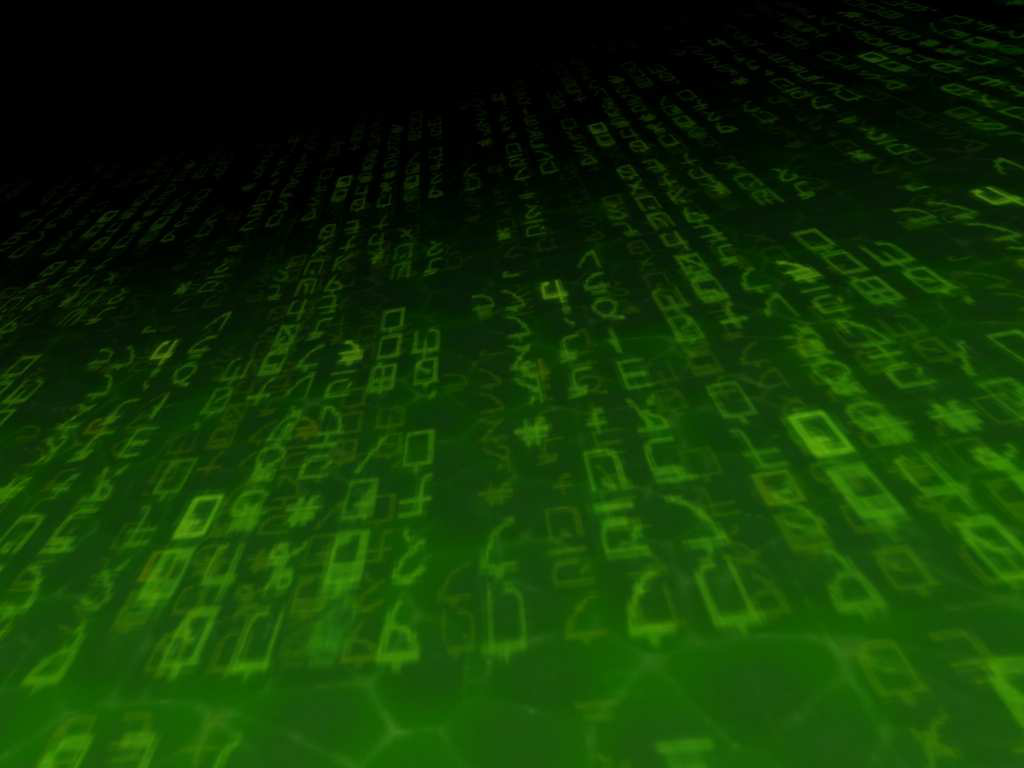
\includegraphics[width=0.2\linewidth]{pgp.png}
\end{figure}
\end{frame}

\begin{frame}
\frametitle{Protocols}
\begin{itemize}
\item SSH (Secure Shell)
\item DSS (Digital satellite system)
\item SET (Secure electronic transaction)
\item SSL (Secure sockets layer) 
\item TLS (Transport layer security)
\item OpenPGP
\end{itemize}
\end{frame}

%------------------------------------------------
\begin{frame}
\frametitle{SSH}
SSH uses public-key cryptography to authenticate the remote computer and allow it to authenticate the user, if necessary.
\begin{itemize}
\item Use automatically generated public-private key pairs to simply encrypt a network connection, and then use password authentication to log on.
\item Use a manually generated public-private key pair to perform the authentication, allowing users or programs to log in without having to specify a password.
\end{itemize}
SSH only verifies whether the same person offering the public key also owns the matching private key.
\begin{figure}
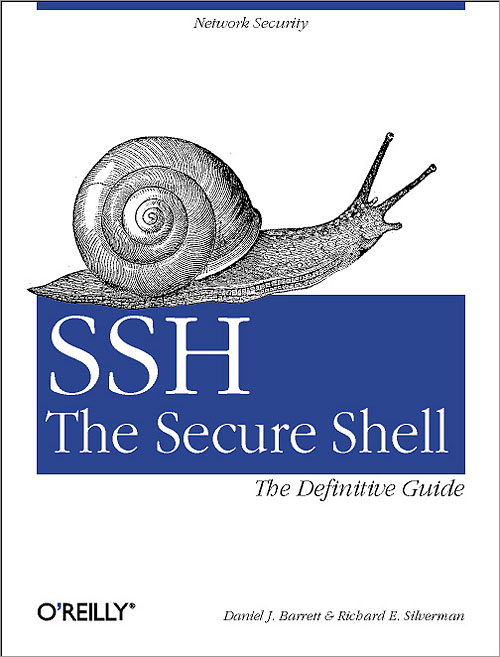
\includegraphics[width=0.1\linewidth]{librossh.jpg}
\end{figure}
\end{frame}


\begin{frame}
\frametitle{Acceptance and revision methods}
\framesubtitle{Standard organizations}
\begin{itemize}
\item ANSI (American National Standards Institute)
\begin{figure}

\includegraphics[width=0.3\linewidth]{ansi.png}
\end{figure}
\item ISO (International Organization for Standardization)
\begin{figure}

\includegraphics[width=0.3\linewidth]{iso.png}
\end{figure}
\item IEEE (Institute of Electrical and Electronics Engineers)
\begin{figure}

\includegraphics[width=0.3\linewidth]{ieee.png}
\end{figure}
\item IETF (Internet Engineering Task Force)
\end{itemize}
\end{frame}

\begin{frame}
\frametitle{Acceptance and revision methods}
\framesubtitle{Criptograph organizations}
\begin{itemize}
\item NSA (National Security Agency)
\item GCHQ (Government Communications Headquarters) UK government
\item Communications Security Establishment (CSE) Canadian intelligence agency.
\begin{figure}

\includegraphics[width=0.3\linewidth]{cse.png}
\end{figure}
\end{itemize}
\end{frame}

\begin{frame}
\framesubtitle{Open efforts}
\begin{itemize}
\item NESSIE (New European Schemes for Signatures, Integrity, and Encryption) (European Union)
\item CrypToolproject (eLearning Program for Cryptography and cryptanalysis)
\begin{figure}

\includegraphics[width=0.3\linewidth]{cryptool.png}
\end{figure}
\item CRYPT REC (Cryptography Research and Evaluation Committee) (Japanese Government)
\end{itemize}
\end{frame}

%----------------------------------------------------------------------------------------

\end{document} 
